\documentclass[tikz]{standalone}

\usepackage[latin1]{inputenc}
\usepackage{tikz}

% GNUPL
\begin{document}
\pagestyle{empty}


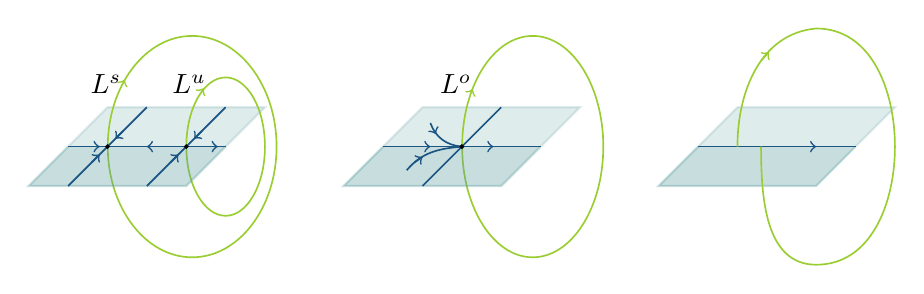
\begin{tikzpicture}
    \draw[color={rgb,255:red,95; green,158; blue,160},thick][fill,  opacity=0.2] (-1.5,3.5) -- (-1,4) -- (1,4) -- (0.5,3.5);
    \draw[semithick,color={rgb,255:red,154; green,205; blue,50}]  (0.5,3.5) ellipse (14.2pt and 25pt);
    \draw[semithick,color={rgb,255:red,154; green,205; blue,50}] (0.075,3.5) ellipse (30.5pt and 40pt);
    \draw[semithick,color={rgb,255:red,154; green,205; blue,50}] [->] (-0.8,4.31) -- (-0.78,4.35);
    \draw[semithick,color={rgb,255:red,154; green,205; blue,50}] [->] (0.2,4.21) -- (0.22,4.24);
    \draw[color={rgb,255:red,95; green,158; blue,160},thick,] [fill,  opacity=0.35] (0.5,3.5) -- (0,3) --(-2,3) -- (-1.5,3.5);
    \draw[semithick, color={rgb,255:red,27; green,85; blue,131}][->] (-0.8,3.7) -- (-0.9,3.6);
    \draw[semithick, color={rgb,255:red,27; green,85; blue,131}][->] (-1.2,3.3) -- (-1.1,3.4);
    \draw[semithick, color={rgb,255:red,27; green,85; blue,131}] (-1.5,3.5) -- (0.5,3.5);
    \draw[semithick, color={rgb,255:red,27; green,85; blue,131}](-1.5,3) -- (-0.5,4);
    \draw[semithick, color={rgb,255:red,27; green,85; blue,131}](-0.5,3) -- (0.5,4);
    \draw[semithick, color={rgb,255:red,27; green,85; blue,131}][->] (0.2,3.7) -- (0.1,3.6);
    \draw[semithick, color={rgb,255:red,27; green,85; blue,131}][->] (-0.2,3.3) -- (-0.1,3.4);
    \draw[semithick, color={rgb,255:red,27; green,85; blue,131}][<-] (-1.1,3.5) -- (-1.2,3.5);
    \draw[semithick, color={rgb,255:red,27; green,85; blue,131}][<-] (-0.5,3.5) -- (-0,3.5);
    \draw[semithick, color={rgb,255:red,27; green,85; blue,131}][<-] (0.4,3.5) -- (0.3,3.5);

    \coordinate [label=0:$L^s$] (8) at (-1.34,4.3);
    \coordinate [label=0:$L^u$] (8) at (-0.3,4.3);
    \draw[semithick][fill] (-01,3.5) ellipse (0.5pt and 0.5pt);
    \draw[semithick][fill] (0,3.5) ellipse (0.5pt and 0.51pt);

    %#2
    \draw[color={rgb,255:red,95; green,158; blue,160},thick][fill,  opacity=0.2] (2.5,3.5) -- (3,4) -- (5,4) -- (4.5,3.5);
    \draw[semithick,color={rgb,255:red,154; green,205; blue,50}] (4.4,3.5) ellipse (25.5pt and 40pt);
    \draw[color={rgb,255:red,95; green,158; blue,160},thick,] [fill,  opacity=0.35] (4.5,3.5) -- (4,3) --(2,3) -- (2.5,3.5);
    \draw[semithick, color={rgb,255:red,27; green,85; blue,131}] (2.5,3.5) -- (4.5,3.5);
    \draw[semithick, color={rgb,255:red,27; green,85; blue,131}][->] (3,3.5) -- (3.1,3.5);
    \draw[semithick, color={rgb,255:red,27; green,85; blue,131}][->] (3.8,3.5) -- (3.9,3.5);
    \draw[semithick, color={rgb,255:red,27; green,85; blue,131}] (3,3) -- (4,4);
    \draw[color={rgb,255:red,27; green,85; blue,131}, semithick] (3.1,3.8) to [out=-70,in=175] (3.5,3.5);
    \draw[color={rgb,255:red,27; green,85; blue,131}, semithick] (2.8,3.2) to [out=50,in=-175] (3.5,3.5);
    \draw[semithick, color={rgb,255:red,27; green,85; blue,131}][->] (3.15,3.7) -- (3.17,3.66);
    \draw[semithick, color={rgb,255:red,27; green,85; blue,131}][->] (2.9,3.3) -- (3,3.37);
    \draw[semithick,color={rgb,255:red,154; green,205; blue,50}] [->] (3.63,4.21) -- (3.64,4.23);
    \draw[semithick][fill] (3.5,3.5) ellipse (0.5pt and 0.5pt);
    \coordinate [label=0:$L^o$] (8) at (3.1,4.3);

    %#3
    \draw[color={rgb,255:red,95; green,158; blue,160},thick][fill,  opacity=0.2] (6.5,3.5) -- (7,4) -- (9,4) -- (8.5,3.5);
    \draw[color={rgb,255:red,95; green,158; blue,160},thick,] [fill,  opacity=0.35] (8.5,3.5) -- (8,3) --(6,3) -- (6.5,3.5);
    \draw[semithick, color={rgb,255:red,27; green,85; blue,131}] (6.5,3.5) -- (8.5,3.5);
    \draw[semithick, color={rgb,255:red,27; green,85; blue,131}][->] (7.8,3.5) -- (8,3.5);
    \draw[color={rgb,255:red,154; green,205; blue,50}, semithick] (7,3.5) to [out=90,in=-175] (8,5) to [out=0,in=90] (9,3.5) to [out=-90,in=0] (8,2) to [out=180,in=-90] (7.3,3.5);
    \draw[semithick,color={rgb,255:red,154; green,205; blue,50}] [->] (7.3,4.59) -- (7.4,4.7);
\end{tikzpicture}


\end{document}